\documentclass[../DoAn.tex]{subfiles}
\usepackage{float}
\usepackage{tabularx}
\usepackage{array}
\usepackage{ragged2e}
\usepackage{needspace}

\begin{document}

% ============================================================
\section{Kiến trúc tổng thể hệ thống}
\label{section:3.1}

Hệ thống quản lý chuỗi nhà hàng được thiết kế theo kiến trúc đa tầng (Multi-tier Architecture),
kết hợp mô hình \textbf{MVC (Model -- View -- Controller)} và hướng dịch vụ.
Kiến trúc đảm bảo tách biệt rõ ràng giữa giao diện, xử lý nghiệp vụ và quản lý dữ liệu, giúp hệ thống dễ mở rộng,
dễ bảo trì và triển khai trên nhiều chi nhánh.

\subsection{Tổng quan kiến trúc}

Hệ thống được chia thành ba tầng chính. Sơ đồ kiến trúc tổng thể được trình bày như sau.

\begin{figure}[H]
    \centering
    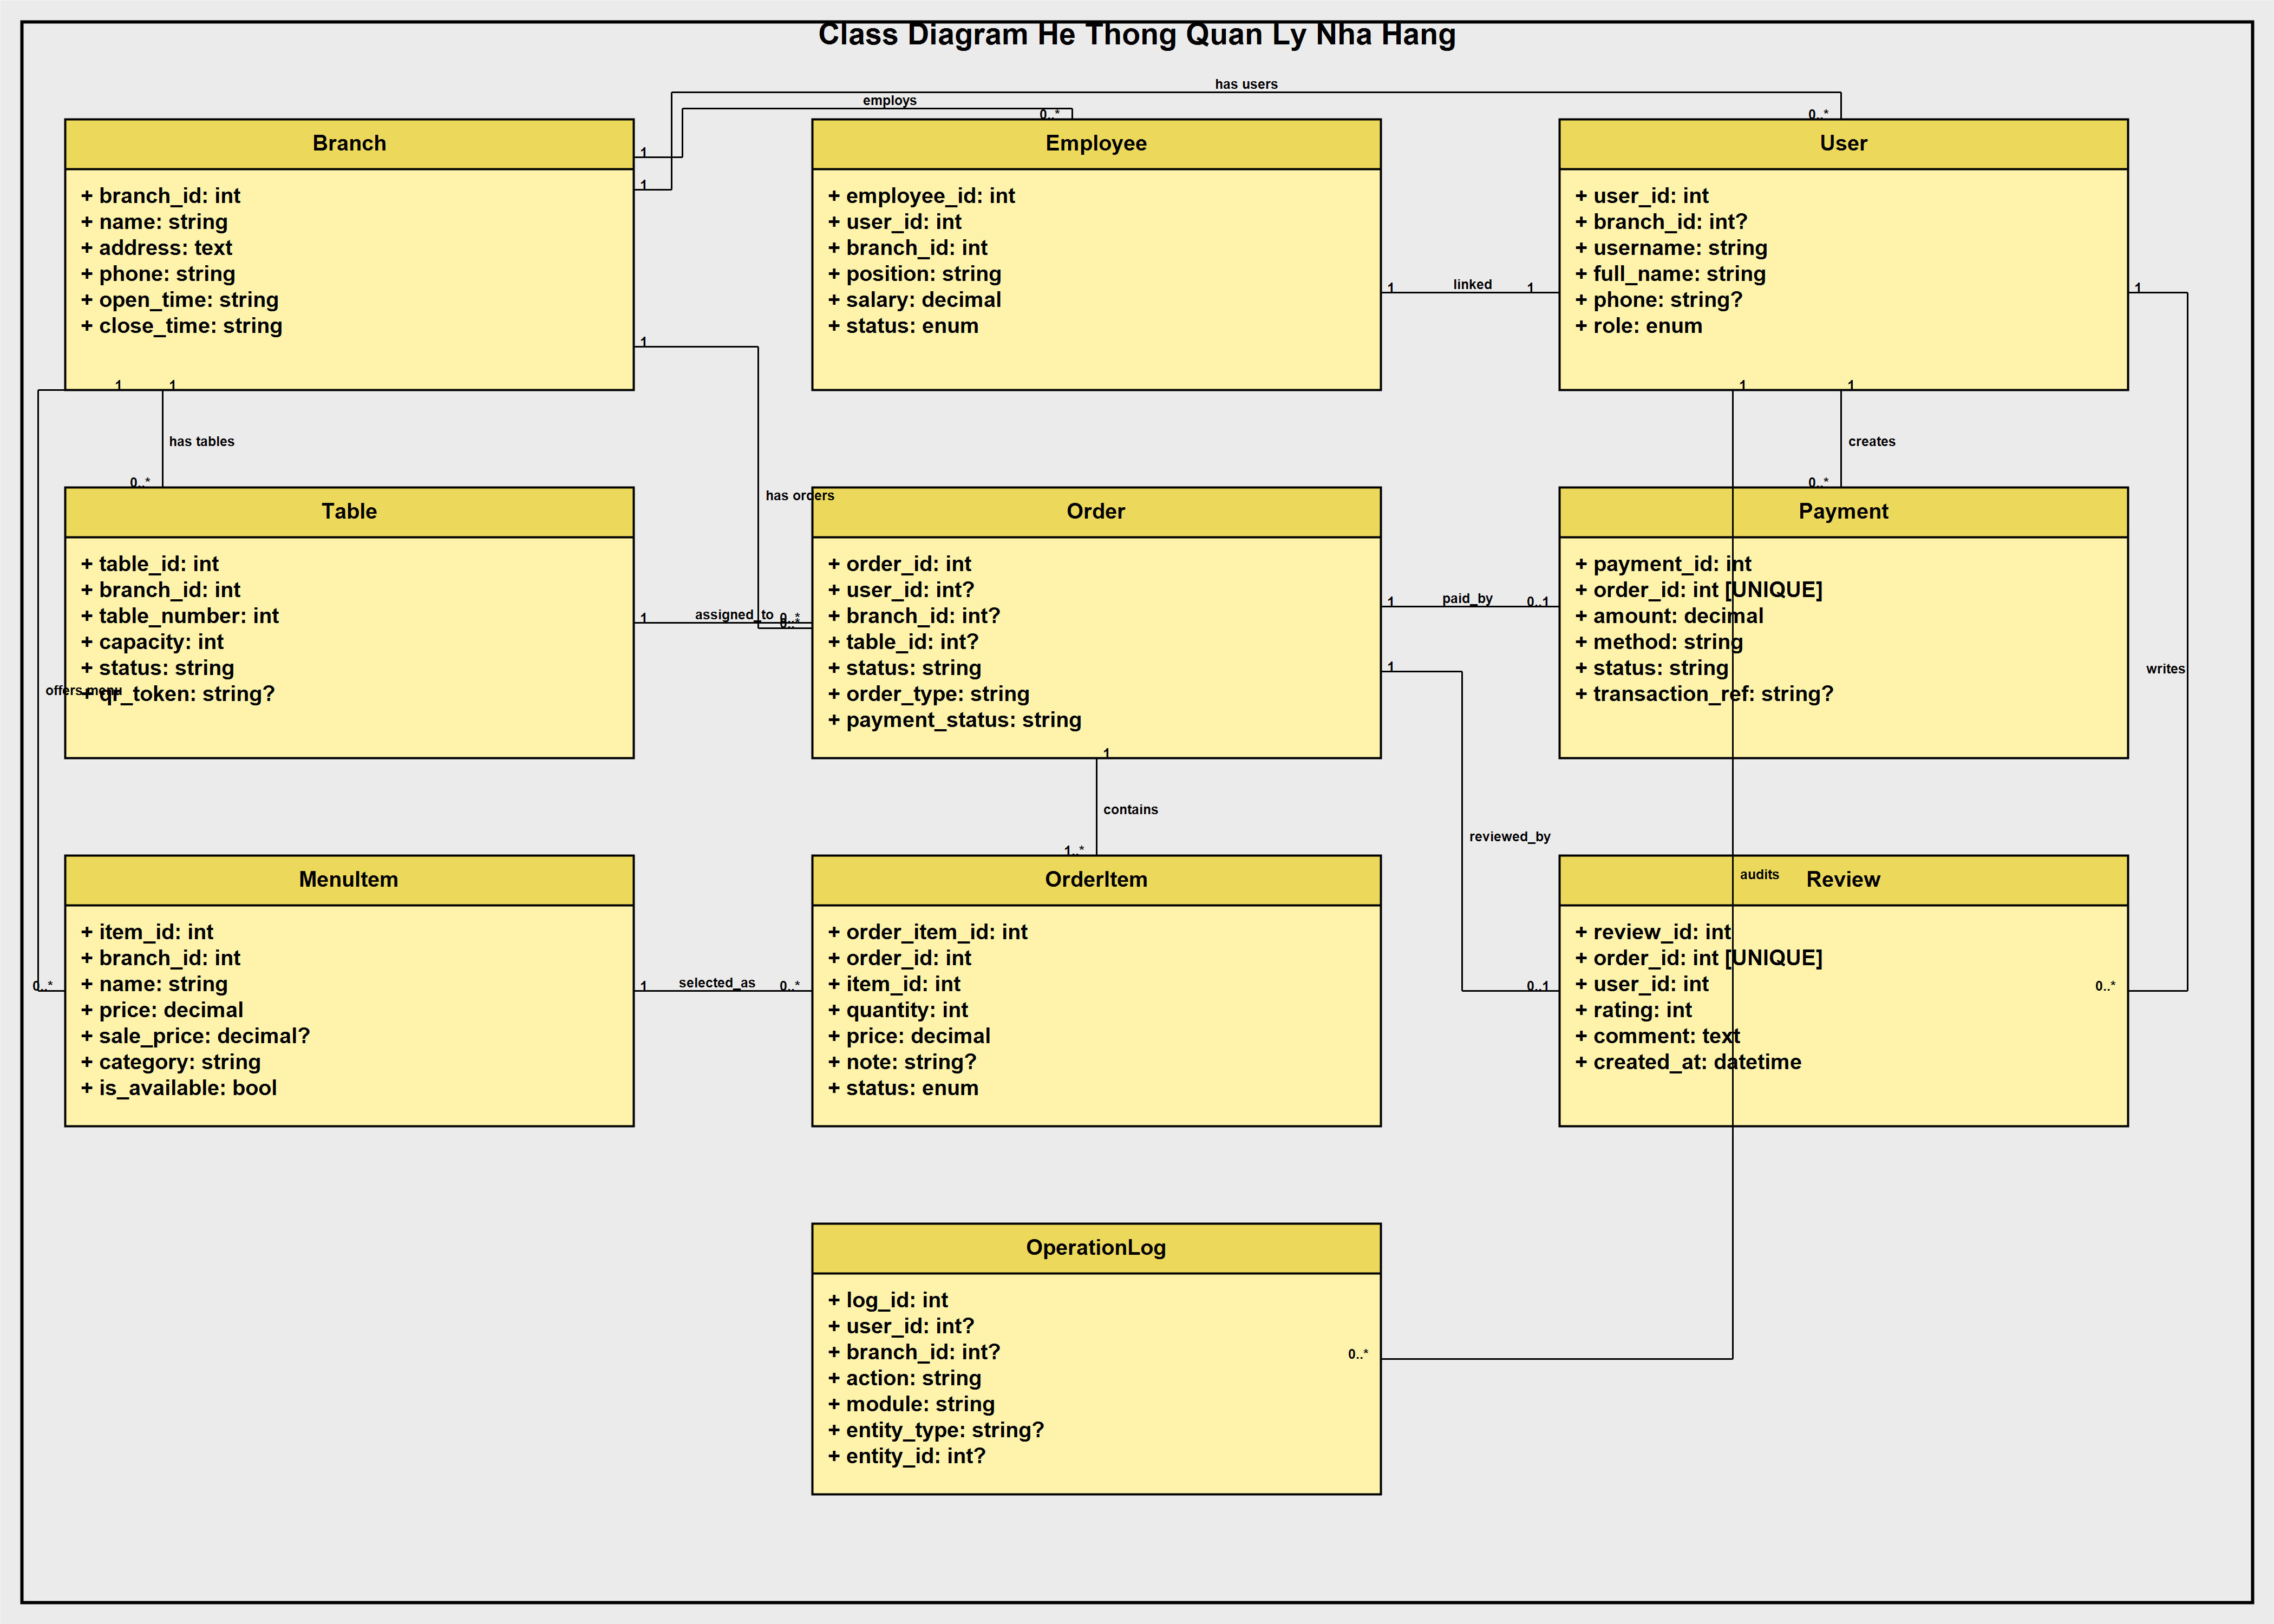
\includegraphics[width=\textwidth]{Chuong/BDQH.png}
    \caption{Sơ đồ kiến trúc đa tầng kết hợp MVC}
    \label{fig:architecture-mvc}
\end{figure}

Hình~\ref{fig:architecture-mvc} thể hiện ba tầng View, Controller và Model cùng luồng phụ thuộc giữa chúng:

\begin{itemize}
    \item \textit{Tầng trình bày (Frontend)}
    Phát triển bằng Vue.js 3 kết hợp Element Plus, là nơi tương tác trực tiếp với khách hàng, nhân viên phục vụ, nhân viên bếp, quản lý chi nhánh và admin hệ thống.
    Frontend giao tiếp với Backend qua API (HTTP/HTTPS) và WebSocket khi cần đồng bộ realtime.

    \item \textit{Tầng ứng dụng (Backend)}
    Xây dựng bằng Node.js và Express, chịu trách nhiệm xử lý toàn bộ logic nghiệp vụ UC01--UC17, gồm:
    \begin{itemize}
        \item Quản lý đặt bàn, kiểm tra bàn trống theo buffer giữ chỗ 2 giờ, tự động phân bàn và ghép bàn liền kề.
        \item Tạo phiên phục vụ (\texttt{orders}), gọi món, đồng bộ trạng thái chế biến giữa phục vụ và bếp.
        \item Xử lý no-show (quá 15 phút sau giờ đặt chưa check-in), hủy đặt bàn và giải phóng bàn.
        \item Tổng hợp hóa đơn, thanh toán (tiền mặt, chuyển khoản, Momo, VietQR).
        \item Quản lý menu, chi nhánh, nhân sự và tài khoản.
        \item Thống kê doanh thu, đánh giá khách hàng.
        \item Phân quyền theo vai trò (\texttt{role}) và phạm vi chi nhánh.
    \end{itemize}

    \item \textit{Tầng dữ liệu (Database)}
    Sử dụng PostgreSQL, lưu trữ tập trung các bảng \texttt{users}, \texttt{branches}, \texttt{tables}, \texttt{orders},
    \texttt{order\_tables}, \texttt{order\_items}, \texttt{menu\_items}, \texttt{payments}, \texttt{reviews}, \texttt{employees}.
\end{itemize}

\subsection{Kiến trúc triển khai}

Kiến trúc triển khai tổng thể trên Hình~\ref{fig:architecture-mvc} gồm các thành phần chính:

\begin{itemize}
    \item Client (Browser) -- giao diện theo từng vai trò người dùng.
    \item API Server -- tiếp nhận yêu cầu, kiểm tra xác thực/phân quyền và điều phối xử lý nghiệp vụ.
    \item Lớp nghiệp vụ (Service) -- hiện thực các quy tắc đặt bàn, vận hành phục vụ, thanh toán và quản trị.
    \item Lớp truy cập dữ liệu (ORM) -- ánh xạ thực thể và thực thi truy vấn trên CSDL.
    \item Cơ sở dữ liệu quan hệ -- lưu trữ dữ liệu và ràng buộc toàn vẹn.
    \item Kênh realtime -- đồng bộ trạng thái món ăn giữa bếp và phục vụ theo chi nhánh (UC08).
\end{itemize}

Luồng xử lý điển hình: Client gửi yêu cầu $\rightarrow$ kiểm tra xác thực/phân quyền
$\rightarrow$ xử lý nghiệp vụ $\rightarrow$ truy cập CSDL $\rightarrow$ phản hồi kết quả.

\subsection{Luồng tương tác tổng quát}

\begin{enumerate}
    \item \textbf{Đặt bàn (Customer $\rightarrow$ Waiter)}
    Khách gửi yêu cầu $\rightarrow$ hệ thống kiểm tra xung đột theo khoảng
    $[\mathit{arrival\_time},\; \mathit{expected\_end\_time}]$ với $\mathit{expected\_end\_time}=\mathit{arrival\_time}+2\,\mathrm{h}$
    $\rightarrow$ tạo phiên đặt bàn và xác nhận giữ chỗ
    $\rightarrow$ nhân viên tiếp nhận khách khi đến và cập nhật trạng thái bàn.
    Nếu quá 15 phút sau giờ đặt mà chưa check-in, tác vụ nền xử lý no-show và nhả bàn.
    \item \textbf{Gọi món và bếp xử lý (Waiter/Kitchen)}
    Nhân viên hoặc khách chọn món $\rightarrow$ bếp nhận danh sách món cần chế biến
    $\rightarrow$ cập nhật trạng thái chế biến $\rightarrow$ phục vụ giao món (đồng bộ realtime).
    \item \textbf{Thanh toán}
    Hệ thống tổng hợp hóa đơn $\rightarrow$ ghi nhận thanh toán
    $\rightarrow$ cập nhật trạng thái phiên phục vụ $\rightarrow$ xuất hóa đơn.
    \item \textbf{Quản lý chi nhánh}
    Quản lý cập nhật menu, thông tin chi nhánh, xem báo cáo doanh thu và đánh giá khách hàng.
    \item \textbf{Quản trị toàn hệ thống}
    Admin quản lý chi nhánh, tài khoản, phân quyền và báo cáo tổng hợp.
\end{enumerate}

\subsection{Mối quan hệ giữa các thành phần}

\begin{itemize}
    \item \textit{Separation of Concerns}: Mỗi tầng đảm nhiệm một vai trò độc lập (View / Controller / Service / Model).
    \item \textit{Loose Coupling}: Frontend chỉ phụ thuộc API contract, không truy cập trực tiếp CSDL.
    \item \textit{Role-based Access}: Phân quyền theo \texttt{users.role} và phạm vi \texttt{branch\_id}.
    \item \textit{Real-time synchronization}: Trạng thái món ăn được cập nhật liên tục qua WebSocket theo chi nhánh.
    \item \textit{Interval-based booking}: Giữ chỗ bàn dựa trên khoảng thời gian có hạn (buffer 2 giờ), không chỉ mốc \textit{arrival\_time} đơn lẻ.
\end{itemize}

\subsection{Định hướng mở rộng}

\begin{itemize}
    \item Tích hợp thêm cổng thanh toán (VNPay, ví điện tử) end-to-end phía khách hàng.
    \item Cấu hình buffer theo chi nhánh hoặc theo khung giờ cao điểm.
    \item Mở rộng kênh WebSocket cho toàn hệ thống đa chi nhánh.
    \item Hỗ trợ mobile app hoặc PWA dùng chung API hiện có.
    \item Phân tích doanh thu bằng công cụ BI khi dữ liệu tích lũy đủ lớn.
\end{itemize}

% ============================================================
\section{Biểu đồ trình tự}
\label{section:3.2}

Biểu đồ trình tự mô tả tương tác giữa các tác nhân (khách hàng, nhân viên, bếp, hệ thống)
theo thời gian cho ba quy trình nghiệp vụ trọng tâm, bám sát luồng UC05--UC07 (đặt bàn, gọi món) và UC11 (thanh toán).

Quy trình đặt bàn và kiểm tra buffer 2 giờ được mô tả như sau.

\begin{figure}[H]
    \centering
    \includegraphics[width=\textwidth]{Chuong/Sequence1.png}
    \caption{Biểu đồ trình tự: Quy trình đặt bàn (kiểm tra buffer 2 giờ)}
    \label{fig:seq-booking}
\end{figure}

Hình~\ref{fig:seq-booking} mô tả khách chọn chi nhánh, thời gian và số khách; hệ thống kiểm tra bàn trống
theo quy tắc giữ chỗ theo khoảng thời gian $[\mathit{arrival\_time},\; \mathit{arrival\_time}+2\,\mathrm{h}]$,
sau đó tạo phiên đặt bàn và ghi nhận thời điểm kết thúc giữ bàn dự kiến.
Nhân viên check-in khi khách đến; nếu quá 15 phút không đến, hệ thống xử lý no-show theo quy định.

Quy trình gọi món và phục vụ được mô tả như sau.

\begin{figure}[H]
    \centering
    \includegraphics[width=\textwidth]{Chuong/Sequence2.png}
    \caption{Biểu đồ trình tự: Quy trình gọi món và phục vụ}
    \label{fig:seq-order}
\end{figure}

Hình~\ref{fig:seq-order} thể hiện luồng thêm \texttt{order\_items}, gửi yêu cầu xuống bếp,
cập nhật trạng thái món và thông báo realtime tới màn hình phục vụ.

Quy trình thanh toán và xuất hoá đơn được mô tả như sau.

\begin{figure}[H]
    \centering
    \includegraphics[width=\textwidth]{Chuong/Sequence3.png}
    \caption{Biểu đồ trình tự: Quy trình thanh toán và xuất hoá đơn}
    \label{fig:seq-payment}
\end{figure}

Hình~\ref{fig:seq-payment} mô tả tổng hợp bill, khởi tạo thanh toán, xác nhận giao dịch
và cập nhật trạng thái phiên phục vụ sau khi thanh toán thành công.

% ============================================================
\section{Thiết kế cơ sở dữ liệu}
\label{section:3.4}

Phần này trình bày lược đồ quan hệ và đặc tả chi tiết các bảng dữ liệu của hệ thống.
Các thực thể nghiệp vụ chính (User, Branch, Table, MenuItem, Order, OrderItem, Payment, Review,...)
và mối quan hệ giữa chúng được thể hiện trên lược đồ quan hệ dưới đây.

\begin{figure}[H]
    \centering
    \includegraphics[width=1.5\textwidth,angle=-90]{Chuong/database.png}
    \caption{Lược đồ quan hệ của cơ sở dữ liệu}
    \label{fig:erd}
\end{figure}

Hình~\ref{fig:erd} mô tả sơ đồ cơ sở dữ liệu tổng thể gồm 10 bảng: 7 bảng lõi
(users, branches, tables, orders, order\_tables, order\_items, menu\_items) và 3 bảng phụ trợ
(payments, reviews, employees) phục vụ thanh toán, đánh giá và nhân sự.
Mỗi \texttt{orders} là một phiên phục vụ (đặt bàn trước, walk-in hoặc tại bàn):
lưu thời gian đến, thời gian dự kiến kết thúc giữ bàn, số khách, tổng tiền và trạng thái thanh toán; chi tiết món nằm ở \texttt{order\_items}.
Trường \texttt{order\_type} phân loại kênh phục vụ; trường \texttt{status} mô tả trạng thái phiên theo vòng đời nghiệp vụ.
Trên sơ đồ, một chi nhánh có nhiều bàn, món ăn, nhân viên và phiên phục vụ; một \texttt{orders} gồm nhiều \texttt{order\_items},
có thể liên kết nhiều \texttt{tables} qua \texttt{order\_tables} khi ghép bàn, và có tối đa một \texttt{payments} cùng một \texttt{reviews}.
Các quan hệ được ràng buộc bằng khóa ngoại nhằm đảm bảo tính toàn vẹn tham chiếu.
Đặc tả chi tiết từng bảng trên Hình~\ref{fig:erd} được trình bày như sau.

\subsubsection{Bảng \texttt{users}}

Bảng \texttt{users} lưu tài khoản đăng nhập của mọi vai trò. Trường \texttt{role} xác định quyền truy cập hệ thống
(admin, manager, waiter, kitchen, user); khác với \texttt{employees.position} (chức danh nhân sự tại chi nhánh).
Trong thiết kế hiện tại, \texttt{user\_id} là khóa chính nội bộ để liên kết dữ liệu giữa các bảng; hệ thống không yêu cầu mã hóa trường định danh này ở mức cơ sở dữ liệu.

\needspace{16\baselineskip}
\begin{table}[H]
\centering
\renewcommand{\arraystretch}{1.3}
\small
\begin{tabularx}{\textwidth}{|c|>{\RaggedRight\arraybackslash}p{2.9cm}|>{\Centering\arraybackslash}p{2.2cm}|>{\Centering\arraybackslash}p{1.3cm}|>{\Centering\arraybackslash}p{2.2cm}|>{\RaggedRight\arraybackslash}X|}
\hline
\textbf{STT} & \textbf{Tên thuộc tính} & \textbf{Kiểu dữ liệu} & \textbf{Kích thước} & \textbf{Ràng buộc} & \textbf{Giải thích} \\
\hline
1 & user\_id & INTEGER & - & PK & Định danh duy nhất của người dùng. \\ \hline
2 & branch\_id & INTEGER & - & FK, NULL & Chi nhánh làm việc của nhân viên/quản lý. \\ \hline
3 & username & VARCHAR & 30 & NOT NULL, UNIQUE & Tên đăng nhập (3--30 ký tự, chữ thường/số/\_). \\ \hline
4 & password\_hash & VARCHAR & 60 & NOT NULL & Hash bcrypt (đúng 60 ký tự). \\ \hline
5 & full\_name & VARCHAR & 50 & NOT NULL & Họ và tên (tối đa 50 ký tự). \\ \hline
6 & phone & VARCHAR & 10 & UNIQUE, NULL & SĐT Việt Nam (10 số, bắt đầu 0). \\ \hline
7 & role & ENUM & - & NOT NULL & \texttt{admin}, \texttt{manager}, \texttt{waiter}, \texttt{kitchen}, \texttt{user}. \\ \hline
8 & avatar\_url & TEXT & - & NULL & Ảnh đại diện. \\ \hline
9 & is\_active & BOOLEAN & - & NOT NULL & Tài khoản còn hoạt động hay không. \\ \hline
10 & locked & BOOLEAN & - & NOT NULL & Tài khoản bị khóa hay không (chống spam đặt bàn). \\ \hline
11 & created\_at & TIMESTAMP & - & NOT NULL & Thời điểm tạo tài khoản. \\ \hline
\end{tabularx}
\caption{Mô tả bảng \texttt{users}}
\end{table}

Về bảo mật truy cập, hệ thống sử dụng token xác thực để nhận diện người dùng ở mỗi request; quyền thao tác được kiểm soát theo \texttt{role} và phạm vi dữ liệu hợp lệ. Do đó, nguy cơ truy cập trái phép được xử lý bằng cơ chế xác thực/phân quyền ở tầng ứng dụng thay vì phụ thuộc vào việc mã hóa \texttt{user\_id}.

\subsubsection{Bảng \texttt{branches}}

\needspace{16\baselineskip}
\begin{table}[H]
\centering
\renewcommand{\arraystretch}{1.3}
\small
\begin{tabularx}{\textwidth}{|c|>{\RaggedRight\arraybackslash}p{2.9cm}|>{\Centering\arraybackslash}p{2.2cm}|>{\Centering\arraybackslash}p{1.3cm}|>{\Centering\arraybackslash}p{2.2cm}|>{\RaggedRight\arraybackslash}X|}
\hline
\textbf{STT} & \textbf{Tên thuộc tính} & \textbf{Kiểu dữ liệu} & \textbf{Kích thước} & \textbf{Ràng buộc} & \textbf{Giải thích} \\
\hline
1 & branch\_id & INTEGER & - & PK & Định danh chi nhánh. \\ \hline
2 & name & VARCHAR & 50 & NOT NULL & Tên chi nhánh. \\ \hline
3 & address & TEXT & - & NOT NULL & Địa chỉ chi tiết. \\ \hline
4 & phone & VARCHAR & 10 & NOT NULL & SĐT liên hệ (10 số). \\ \hline
5 & open\_time & VARCHAR & 8 & NULL & Giờ mở cửa (HH:MM). \\ \hline
6 & close\_time & VARCHAR & 8 & NULL & Giờ đóng cửa (HH:MM). \\ \hline
7 & image\_url & TEXT & - & NULL & Ảnh minh họa chi nhánh. \\ \hline
8 & latitude & DECIMAL & 10,7 & NULL & Vĩ độ (bản đồ, độ chính xác $\approx$1\,cm tại VN). \\ \hline
9 & longitude & DECIMAL & 10,7 & NULL & Kinh độ (bản đồ). \\ \hline
10 & is\_active & BOOLEAN & - & NOT NULL & Chi nhánh còn hoạt động. \\ \hline
11 & created\_at & TIMESTAMP & - & NOT NULL & Thời điểm tạo. \\ \hline
12 & updated\_at & TIMESTAMP & - & NULL & Thời điểm cập nhật gần nhất. \\ \hline
\end{tabularx}
\caption{Mô tả bảng \texttt{branches}}
\end{table}

Bảng \texttt{branches} là trung tâm phân vùng dữ liệu theo chi nhánh, liên kết trực tiếp với
\texttt{tables}, \texttt{menu\_items}, \texttt{orders} và \texttt{employees}.
Đánh giá khách hàng (\texttt{reviews}) gắn gián tiếp qua \texttt{orders.branch\_id}.

\subsubsection{Bảng \texttt{tables}}

\needspace{16\baselineskip}
\begin{table}[H]
\centering
\renewcommand{\arraystretch}{1.3}
\small
\begin{tabularx}{\textwidth}{|c|>{\RaggedRight\arraybackslash}p{2.9cm}|>{\Centering\arraybackslash}p{2.2cm}|>{\Centering\arraybackslash}p{1.3cm}|>{\Centering\arraybackslash}p{2.2cm}|>{\RaggedRight\arraybackslash}X|}
\hline
\textbf{STT} & \textbf{Tên thuộc tính} & \textbf{Kiểu dữ liệu} & \textbf{Kích thước} & \textbf{Ràng buộc} & \textbf{Giải thích} \\
\hline
1 & table\_id & INTEGER & - & PK & Định danh bàn. \\ \hline
2 & branch\_id & INTEGER & - & FK, NOT NULL & Chi nhánh sở hữu bàn. \\ \hline
3 & table\_number & INTEGER & - & NOT NULL & Số thứ tự bàn trong chi nhánh. \\ \hline
4 & capacity & INTEGER & - & NOT NULL & Sức chứa tối đa. \\ \hline
5 & status & VARCHAR & 15 & NOT NULL & \texttt{available}, \texttt{pre-ordered}, \texttt{occupied}, \texttt{cleaning}. \\ \hline
6 & qr\_token & VARCHAR & 32 & UNIQUE, NULL & Mã QR tĩnh (32 ký tự hex) để khách quét gọi món. \\ \hline
7 & created\_at & TIMESTAMP & - & NOT NULL & Thời điểm tạo. \\ \hline
\end{tabularx}
\caption{Mô tả bảng \texttt{tables}}
\end{table}

\subsubsection{Bảng \texttt{menu\_items}}

\needspace{16\baselineskip}
\begin{table}[H]
\centering
\renewcommand{\arraystretch}{1.3}
\small
\begin{tabularx}{\textwidth}{|c|>{\RaggedRight\arraybackslash}p{2.9cm}|>{\Centering\arraybackslash}p{2.2cm}|>{\Centering\arraybackslash}p{1.3cm}|>{\Centering\arraybackslash}p{2.2cm}|>{\RaggedRight\arraybackslash}X|}
\hline
\textbf{STT} & \textbf{Tên thuộc tính} & \textbf{Kiểu dữ liệu} & \textbf{Kích thước} & \textbf{Ràng buộc} & \textbf{Giải thích} \\
\hline
1 & item\_id & INTEGER & - & PK & Định danh món ăn. \\ \hline
2 & branch\_id & INTEGER & - & FK, NOT NULL & Chi nhánh quản lý món. \\ \hline
3 & name & VARCHAR & 50 & NOT NULL & Tên món ăn. \\ \hline
4 & description & TEXT & - & NULL & Mô tả ngắn. \\ \hline
5 & price & DECIMAL & 10,2 & NOT NULL & Giá niêm yết (VNĐ). \\ \hline
6 & category & VARCHAR & 15 & NOT NULL & Danh mục (Khai vị, Món chính,...). \\ \hline
7 & is\_available & BOOLEAN & - & NOT NULL & Món còn phục vụ hay không. \\ \hline
8 & sale\_price & DECIMAL & 10,2 & NULL & Giá khuyến mãi (nếu có). \\ \hline
9 & is\_featured & BOOLEAN & - & NOT NULL & Món nổi bật trên trang chủ/menu. \\ \hline
10 & image\_url & TEXT & - & NULL & Đường dẫn hình ảnh. \\ \hline
11 & created\_at & TIMESTAMP & - & NOT NULL & Thời điểm tạo. \\ \hline
\end{tabularx}
\caption{Mô tả bảng \texttt{menu\_items}}
\end{table}

\subsubsection{Bảng \texttt{orders}}

Bảng trung tâm nghiệp vụ: mỗi dòng là một phiên phục vụ (đặt bàn trước, walk-in hoặc tại bàn),
gồm thông tin khách, bàn, món (qua \texttt{order\_items}) và thanh toán.
\texttt{payment\_status} phản ánh trạng thái tổng quát trên phiên; chi tiết giao dịch nằm ở bảng \texttt{payments}.
Trường \texttt{expected\_end\_time} hỗ trợ kiểm tra xung đột giữ chỗ theo buffer 2 giờ;
\texttt{checked\_in\_at} ghi nhận thời điểm nhân viên tiếp nhận khách thực tế.
Khi khách đặt bàn hoặc nhân viên tạo walk-in, hệ thống gán mỗi phiên một khoảng chiếm bàn
$\mathit{hold\_start}=\mathit{arrival\_time}$, $\mathit{hold\_end}=\mathit{expected\_end\_time}=\mathit{arrival\_time}+2\,\text{giờ}$.
Một bàn khả dụng tại thời điểm $T$ nếu không tồn tại phiên active mà khoảng giữ bàn giao với $[T,\; T+2\,\text{giờ}]$;
việc kiểm tra và gán bàn được thực hiện trong giao dịch, với nhóm đông có thể ghép nhiều bàn liền kề qua \texttt{order\_tables}.

\needspace{20\baselineskip}
\begin{table}[H]
\centering
\renewcommand{\arraystretch}{1.15}
\footnotesize
\setlength{\tabcolsep}{4pt}
\begin{tabularx}{\textwidth}{|c|>{\RaggedRight\arraybackslash}p{2.9cm}|>{\Centering\arraybackslash}p{2.2cm}|>{\Centering\arraybackslash}p{1.3cm}|>{\Centering\arraybackslash}p{2.2cm}|>{\RaggedRight\arraybackslash}X|}
\hline
\textbf{STT} & \textbf{Tên thuộc tính} & \textbf{Kiểu dữ liệu} & \textbf{Kích thước} & \textbf{Ràng buộc} & \textbf{Giải thích} \\
\hline
1 & order\_id & INTEGER & - & PK & Định danh phiên/đơn hàng. \\ \hline
2 & user\_id & INTEGER & - & FK, NULL & Khách hàng hoặc nhân viên tạo. \\ \hline
3 & branch\_id & INTEGER & - & FK, NULL & Chi nhánh phát sinh (bắt buộc khi xác nhận phiên). \\ \hline
4 & table\_id & INTEGER & - & FK, NULL & Bàn chính được phân/phục vụ. \\ \hline
5 & arrival\_time & TIMESTAMP & - & NULL & Giờ khách đến hoặc giờ đặt trước. \\ \hline
6 & expected\_end\_time & TIMESTAMP & - & NULL & Thời điểm dự kiến kết thúc giữ bàn ($\mathit{arrival\_time}+2\,\mathrm{h}$). \\ \hline
7 & checked\_in\_at & TIMESTAMP & - & NULL & Thời điểm nhân viên check-in khách vào bàn. \\ \hline
8 & number\_of\_guests & INTEGER & - & NULL & Số lượng khách. \\ \hline
9 & status & VARCHAR & 20 & NOT NULL & \texttt{pending}, \texttt{confirmed}, \texttt{pre-ordered}, \texttt{in\_progress}, \texttt{waiting\_payment}, \texttt{completed}, \texttt{cancelled}, \texttt{no\_show}. \\ \hline
10 & total\_amount & DECIMAL & 10,2 & NULL & Tổng tiền (đồng bộ từ \texttt{order\_items}). \\ \hline
11 & note & VARCHAR & 200 & NULL & Ghi chú đặt bàn/đơn. \\ \hline
12 & order\_type & VARCHAR & 15 & NOT NULL & \texttt{reservation}, \texttt{walk\_in}, \texttt{dine\_in}. \\ \hline
13 & payment\_status & VARCHAR & 16 & NOT NULL & \texttt{unpaid}, \texttt{pending}, \texttt{succeeded}, \texttt{failed}, \texttt{canceled}. \\ \hline
14 & booking\_group\_id & VARCHAR & 36 & NULL & UUID nhóm đặt nhiều bàn cùng lúc. \\ \hline
15 & created\_at & TIMESTAMP & - & NOT NULL & Thời điểm tạo. \\ \hline
\end{tabularx}
\caption{Mô tả bảng \texttt{orders}}
\label{tab:orders}
\end{table}
\normalsize

\subsubsection{Bảng \texttt{order\_tables}}

Bảng liên kết nhiều--nhiều giữa \texttt{orders} và \texttt{tables}, dùng khi ghép nhiều bàn liền kề cho nhóm đông.
Khóa chính ghép (\texttt{order\_id}, \texttt{table\_id}); \texttt{is\_primary} đánh dấu bàn chính hiển thị trên hóa đơn.

\needspace{14\baselineskip}
\begin{table}[H]
\centering
\renewcommand{\arraystretch}{1.3}
\small
\begin{tabularx}{\textwidth}{|c|>{\RaggedRight\arraybackslash}p{2.9cm}|>{\Centering\arraybackslash}p{2.2cm}|>{\Centering\arraybackslash}p{1.3cm}|>{\Centering\arraybackslash}p{2.2cm}|>{\RaggedRight\arraybackslash}X|}
\hline
\textbf{STT} & \textbf{Tên thuộc tính} & \textbf{Kiểu dữ liệu} & \textbf{Kích thước} & \textbf{Ràng buộc} & \textbf{Giải thích} \\
\hline
1 & order\_id & INTEGER & - & PK, FK, NOT NULL & Phiên phục vụ. \\ \hline
2 & table\_id & INTEGER & - & PK, FK, NOT NULL & Bàn được gán trong phiên. \\ \hline
3 & is\_primary & BOOLEAN & - & NOT NULL & Bàn chính của phiên (mặc định bàn đầu tiên). \\ \hline
\end{tabularx}
\caption{Mô tả bảng \texttt{order\_tables}}
\end{table}

\subsubsection{Bảng \texttt{order\_items}}

\needspace{14\baselineskip}
\begin{table}[H]
\centering
\renewcommand{\arraystretch}{1.3}
\small
\begin{tabularx}{\textwidth}{|c|>{\RaggedRight\arraybackslash}p{2.9cm}|>{\Centering\arraybackslash}p{2.2cm}|>{\Centering\arraybackslash}p{1.3cm}|>{\Centering\arraybackslash}p{2.2cm}|>{\RaggedRight\arraybackslash}X|}
\hline
\textbf{STT} & \textbf{Tên thuộc tính} & \textbf{Kiểu dữ liệu} & \textbf{Kích thước} & \textbf{Ràng buộc} & \textbf{Giải thích} \\
\hline
1 & order\_item\_id & INTEGER & - & PK & Định danh dòng món trong đơn. \\ \hline
2 & order\_id & INTEGER & - & FK, NOT NULL & Liên kết đơn hàng. \\ \hline
3 & item\_id & INTEGER & - & FK, NOT NULL & Liên kết món trong menu. \\ \hline
4 & quantity & INTEGER & - & NOT NULL & Số lượng gọi. \\ \hline
5 & price & DECIMAL & 10,2 & NOT NULL & Giá snapshot tại thời điểm gọi món. \\ \hline
6 & note & VARCHAR & 200 & NULL & Ghi chú món (ít cay, không hành,...). \\ \hline
7 & status & ENUM & - & NOT NULL & \texttt{pending}, \texttt{processing}, \texttt{done}, \texttt{served}. \\ \hline
\end{tabularx}
\caption{Mô tả bảng \texttt{order\_items}}
\end{table}

\subsubsection{Bảng \texttt{payments}}

Lưu bản ghi thanh toán chính của mỗi phiên phục vụ. Một \texttt{orders} tương ứng tối đa một \texttt{payments}
(ràng buộc \texttt{order\_id} duy nhất ở tầng nghiệp vụ).

\needspace{16\baselineskip}
\begin{table}[H]
\centering
\renewcommand{\arraystretch}{1.3}
\small
\begin{tabularx}{\textwidth}{|c|>{\RaggedRight\arraybackslash}p{2.9cm}|>{\Centering\arraybackslash}p{2.2cm}|>{\Centering\arraybackslash}p{1.3cm}|>{\Centering\arraybackslash}p{2.2cm}|>{\RaggedRight\arraybackslash}X|}
\hline
\textbf{STT} & \textbf{Tên thuộc tính} & \textbf{Kiểu dữ liệu} & \textbf{Kích thước} & \textbf{Ràng buộc} & \textbf{Giải thích} \\
\hline
1 & payment\_id & INTEGER & - & PK & Định danh thanh toán. \\ \hline
2 & order\_id & INTEGER & - & FK, NOT NULL, UNIQUE & Một phiên \texttt{orders} tối đa một bản ghi thanh toán. \\ \hline
3 & amount & DECIMAL & 10,2 & NOT NULL & Số tiền thanh toán. \\ \hline
4 & method & VARCHAR & 15 & NOT NULL & \texttt{CASH}, \texttt{BANK\_TRANSFER}, \texttt{CARD}, \texttt{WALLET}, \texttt{MOMO}, \texttt{COD}. \\ \hline
5 & status & VARCHAR & 16 & NOT NULL & \texttt{pending}, \texttt{requires\_action}, \texttt{succeeded}, \texttt{failed}, \texttt{canceled}. \\ \hline
6 & transaction\_ref & VARCHAR & 64 & NULL & Mã giao dịch cổng thanh toán. \\ \hline
7 & invoice\_no & VARCHAR & 20 & NULL & Số hoá đơn. \\ \hline
8 & invoice\_issued\_at & TIMESTAMP & - & NULL & Thời điểm xuất hoá đơn. \\ \hline
9 & paid\_at & TIMESTAMP & - & NULL & Thời điểm thanh toán thành công. \\ \hline
10 & created\_at & TIMESTAMP & - & NOT NULL & Thời điểm tạo bản ghi. \\ \hline
\end{tabularx}
\caption{Mô tả bảng \texttt{payments}}
\end{table}

\subsubsection{Bảng \texttt{reviews}}

Lưu đánh giá của khách sau khi hoàn tất phiên phục vụ (UC13). Mỗi \texttt{orders} chỉ nhận tối đa một đánh giá;
khách chỉ được đánh giá phiên thuộc về mình và đã thanh toán/hoàn thành.

\needspace{16\baselineskip}
\begin{table}[H]
\centering
\renewcommand{\arraystretch}{1.3}
\small
\begin{tabularx}{\textwidth}{|c|>{\RaggedRight\arraybackslash}p{2.9cm}|>{\Centering\arraybackslash}p{2.2cm}|>{\Centering\arraybackslash}p{1.3cm}|>{\Centering\arraybackslash}p{2.2cm}|>{\RaggedRight\arraybackslash}X|}
\hline
\textbf{STT} & \textbf{Tên thuộc tính} & \textbf{Kiểu dữ liệu} & \textbf{Kích thước} & \textbf{Ràng buộc} & \textbf{Giải thích} \\
\hline
1 & review\_id & INTEGER & - & PK & Định danh đánh giá. \\ \hline
2 & order\_id & INTEGER & - & FK, NOT NULL, UNIQUE & Một phiên chỉ có một đánh giá. \\ \hline
3 & user\_id & INTEGER & - & FK, NOT NULL & Người đánh giá. \\ \hline
4 & rating & INTEGER & - & NOT NULL & Điểm từ 1--5. \\ \hline
5 & comment & TEXT & - & NOT NULL & Nội dung phản hồi. \\ \hline
6 & created\_at & TIMESTAMP & - & NOT NULL & Thời điểm gửi đánh giá. \\ \hline
\end{tabularx}
\caption{Mô tả bảng \texttt{reviews}}
\end{table}

\subsubsection{Bảng \texttt{employees}}

Hồ sơ nhân sự gắn với tài khoản \texttt{users}. Trường \texttt{position} mô tả chức danh tại chi nhánh
(\texttt{manager}, \texttt{chef}, \texttt{waiter}, \texttt{cashier}), bổ sung cho \texttt{users.role}
dùng phân quyền đăng nhập (ví dụ nhân viên bếp có \texttt{role=kitchen}, \texttt{position=chef}).

\needspace{16\baselineskip}
\begin{table}[H]
\centering
\renewcommand{\arraystretch}{1.3}
\small
\begin{tabularx}{\textwidth}{|c|>{\RaggedRight\arraybackslash}p{2.9cm}|>{\Centering\arraybackslash}p{2.2cm}|>{\Centering\arraybackslash}p{1.3cm}|>{\Centering\arraybackslash}p{2.2cm}|>{\RaggedRight\arraybackslash}X|}
\hline
\textbf{STT} & \textbf{Tên thuộc tính} & \textbf{Kiểu dữ liệu} & \textbf{Kích thước} & \textbf{Ràng buộc} & \textbf{Giải thích} \\
\hline
1 & employee\_id & INTEGER & - & PK & Định danh nhân viên. \\ \hline
2 & user\_id & INTEGER & - & FK, NOT NULL & Tài khoản đăng nhập. \\ \hline
3 & branch\_id & INTEGER & - & FK, NOT NULL & Chi nhánh làm việc. \\ \hline
4 & position & VARCHAR & 20 & NOT NULL & Chức vụ: \texttt{manager}, \texttt{chef}, \texttt{waiter}, \texttt{cashier}. \\ \hline
5 & salary & DECIMAL & 10,2 & NULL & Mức lương. \\ \hline
6 & hire\_date & TIMESTAMP & - & NULL & Ngày vào làm. \\ \hline
7 & status & ENUM & - & NOT NULL & \texttt{active}, \texttt{inactive}, \texttt{on\_leave}. \\ \hline
8 & created\_at & TIMESTAMP & - & NOT NULL & Thời điểm tạo hồ sơ. \\ \hline
9 & updated\_at & TIMESTAMP & - & NOT NULL & Thời điểm cập nhật. \\ \hline
\end{tabularx}
\caption{Mô tả bảng \texttt{employees}}
\end{table}

\end{document}
